% !TeX root = ../tesi.tex

\chapter{Nozioni preliminari}
\label{ch:basics}

Per ogni intero positivo $n$, indico con $[n]$ l'insieme $\{1, 2, \dots, n\}$.

\section{Sistemi di radici}

Sia $V$ uno spazio euclideo, ovvero uno spazio vettoriale reale dotato di un
prodotto scalare $\langle \,\cdot \, , \cdot \,\rangle$ definito positivo.

Per ogni vettore non-nullo $\alpha \in V$, definisco $r_\alpha$
come la riflessione rispetto all'iperpiano ortogonale a $\alpha$,
che si pu\`o scrivere come segue:
\[
    r_\alpha(x) = x - \langle x, \alpha^\vee \rangle \alpha, 
    \qquad \text{dove} \quad \alpha^\vee = \frac{2\alpha}{\langle \alpha, \alpha\rangle}.
\]

\begin{remark}
    Il prodotto scalare permette di identificare $V$ con il suo spazio duale $V^*$.
    Tuttavia, sarebbe meglio pensare ad $\alpha^\vee$ come al funzionale dato da
    \[
        \alpha^\vee =
        2 \frac{\langle \alpha, \cdot \, \rangle}{\langle\alpha,\alpha\rangle}
        \in V^*,
    \]
    e al prodotto $\langle x, \alpha^\vee \rangle$ come all'applicazione del funzionale
    $\alpha^\vee$ al vettore $x$.
\end{remark}

\begin{definition}[Sistema di radici]
    Un \emph{sistema di radici} $\Phi$ in $V$ \`e un sottoinsieme non-vuoto finito di 
    $V \setminus \{ 0 \}$ tale che:
    \begin{enumerate}
        \item $r_\alpha(\Phi) = \Phi$ per ogni $\alpha \in \Phi$;
        \item \label{item:sist_rad_2}
            $\langle \alpha, \beta^\vee \rangle \in \ZZ$ per ogni $\alpha, \beta \in \Phi$;
        \item $\RR \alpha \cap \Phi = \{ \alpha, -\alpha \}$ per ogni $\alpha \in \Phi$.
            % NOTE RR-span, come si scrive?
    \end{enumerate}

    Gli elementi di $\Phi$ si dicono \emph{radici}, 
    mentre gli elementi di 
    \[
        \Phi^\vee \coloneq \{ \alpha^\vee \mid \alpha \in \Phi \}
    \]
    si dicono \emph{coradici}.
\end{definition}

\begin{remark}
    \label{rmk:root_lattice}
    La condizione~\ref{item:sist_rad_2} implica che lo $\ZZ$-span delle radici \`e un reticolo,
    ovvero un sottogruppo additivo \emph{discreto} di $V$.
    % TODO dimostra
\end{remark}

Anche grazie all'Osservazione~\ref{rmk:root_lattice}, definisco 
il reticolo delle radici $\Lambda_\mathrm{root}$
come il reticolo generato dalle radici.

Diciamo inoltre che un reticolo $\Lambda$ \`e un \emph{reticolo dei pesi} per il sistema
di radici $\Phi$ se $\Lambda_\mathrm{root} \subseteq \Lambda$ e vale
\[
    \langle \mu , \alpha^\vee \rangle \in \ZZ ,
    \qquad \text{per ogni $\mu \in \Lambda$ e $\alpha \in \Phi$.}
\]

Fissiamo un iperpiano in $V$ che non contiene alcuna radice in $\Phi$ e chiamiamo le radici
da un lato dell'iperpiano \emph{positive} e quelle dall'altro lato \emph{negative}.
Siano $\Phi^+$ l'insieme delle radici positive e $\Phi^-$ quello delle radici negative.

Una radice positiva si dice \emph{semplice} se non si pu\`o scrivere come somma
di altre radici positive.
Sia $\Sigma$ l'insieme delle radici semplici.
Sia inoltre $I$ un insieme che indicizza le radici semplici.
Quindi possiamo scrivere
$\Sigma = \{ \alpha_i \mid i \in I \}$.


\begin{proposition}
    \label{prop:propriet_radici_semplici}
    L'insieme $\Sigma$ delle radici semplici del sistema di radici $\Phi$ 
    soddisfa le seguenti propriet\`a.
    \begin{enumerate}
        \item Gli elementi di $\Sigma$ sono linearmente indipendenti.
        \item Se $\alpha \in \Sigma$ e $\beta \in \Phi^+$, allora $\beta = \alpha$
            oppure $r_\alpha (\beta) \in \Phi^+$; ovvero $r_\alpha$ permuta
            $\Phi^+ \setminus \{ \alpha \} $.
        \item Se $\alpha$, $\beta$ sono radici distinte in $\Sigma$, allora
            $\langle \alpha, \beta^\vee \rangle \leq 0 $.
        \item Ogni radice positiva si pu\`o scrivere come combinazione lineare a coefficienti
            interi non-negativi di elementi di $\Sigma$.
    \end{enumerate}
\end{proposition}

\begin{proof}
    Si veda \cite[Proposition~20.1]{Bump2013LieGroups}.
\end{proof}

\begin{definition}
    Per ogni sistema di radici $\Phi$, definisco il suo \emph{gruppo di Weyl} $W$ come il
    gruppo generato da $r_\alpha$ al variare di $\alpha \in \Phi$.
\end{definition}

Il gruppo di Weyl si dimostra essere un gruppo di Coxeter, che definiamo adesso.

\begin{definition}

    Sia $G$ un gruppo generato dagli elementi $s_1, s_2, \dots, s_r$.
    Sia inoltre $m_{ij}$ l'ordine dell'elemento $s_i s_j$, per ogni $i,j = 1, \dots, r$.

    Il gruppo $G$ si dice \emph{di Coxeter} se $m_{ii} = 1$ per ogni $i$, ovvero
    i generatori hanno ordine due, e
    \[
        \label{eq:coxeter_pres}
        \bigl\langle s_1, s_2, \dots, s_r \mid (s_i s_j)^{m_{ij}} = 1_G \bigr\rangle
    \]
    \`e una presentazione per $G$, dove gli indici $i$ e $j$ variano tra $1$ e $r$.
    
\end{definition}

\begin{proposition}
    \label{prop:weyl_is_coxeter}
    Il gruppo di Weyl $W$ \`e un gruppo di Coxeter generato dalle riflessioni
    semplici $r_{\alpha_i}$ per $i \in I$.
\end{proposition}

\begin{proof}
    Si veda \cite[Theorem~25.1]{Bump2013LieGroups}.
\end{proof}

Esistono vari sistemi di radici, tuttavia noi considereremo solo i
sistemi di tipo $A$, che descriviamo in seguito.

\begin{example}
    \label{ex:sist_rad_A}
    Fissiamo un intero $\ell$ maggiore di $1$ e un insieme di indici $I = [\ell-1]$.
    Sia $V = \RR^\ell$ e sia $\ee_1, \ee_2, \dots, \ee_\ell$ la sua base canonica.

    Definiamo il sistema di radici $\Phi$ di tipo $A_{\ell-1}$ e le 
    sue radici positive come segue:
    \begin{align*}
        \Phi &= \{ \ee_i - \ee_j \mid i \neq j\}, \\
        \Phi^+ &= \{ \ee_i - \ee_j \mid i < j\}.
    \end{align*}
    Le radici semplici sono $\alpha_i = \ee_i - \ee_{i+1}$ al variare di $i \in I$.

    Non sar\`o troppo rigoroso nella scelta del reticolo dei pesi.
    Solitamente utilizzer\`o $\Lambda = \ZZ^\ell$.
    Tuttavia, a volte \`e comodo che
    i pesi appartengano al sottospazio vettoriale generato dalle radici.
    In tal caso useremo l'immagine della proiezione ortogonale di $\ZZ^\ell$ 
    sul sottospazio generato dalle radici, che \`e equivalente a identificare
    pesi che differiscono solo per un multiplo del vettore $(1, 1, \dots, 1)$.


    La Figura~\ref{fig:ex_sist_rad_A2} mostra il sistema di radici di tipo $A_2$.

    \begin{figure}[htbp]
        \centering
        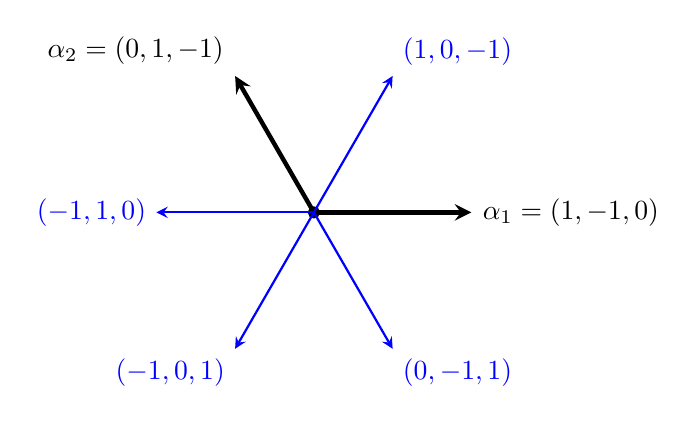
\begin{tikzpicture}[scale=2, >=stealth]

            % Draw a dashed hexagon to highlight the geometry

            % Draw the origin
            \filldraw (0,0) circle (1pt);

            % Draw the simple roots (black)
            \draw[->, ultra thick] (0,0) -- (1,0) 
                node[right] {$\alpha_1 = (1,-1,0)$};
            \draw[->, ultra thick] (0,0) -- (-0.5, {sqrt(3)/2}) 
                node[above left] {$\alpha_2 = (0, 1, -1)$};

            \draw[->, thick, blue] (0,0) -- (0.5, {sqrt(3)/2}) 
                node[above right] {$(1, 0, -1)$};
            \draw[->, thick, blue] (0,0) -- (-1,0) 
                node[left] {$(-1,1,0)$};
            \draw[->, thick, blue] (0,0) -- (0.5, {-sqrt(3)/2}) 
                node[below right] {$(0, -1,1)$};
            \draw[->, thick, blue] (0,0) -- (-0.5, {-sqrt(3)/2}) 
                node[below left] {$(-1,0,1)$};

        \end{tikzpicture}
        \caption{Il sistema di radici di tipo $A_2$, in nero le radici semplici.}
        \label{fig:ex_sist_rad_A2}
    \end{figure}
\end{example}



% \section{Gruppi di Coxeter}
% 
% 
% Sia $W$ un gruppo con identit\`a $1$ 
% e sia $S = \{ s_1, s_2 \dots, s_n \}$ un suo insieme di 
% generatori \emph{di ordine due}, ovvero tali che $s_i^2 = 1$ per ogni $i$ e $1 \notin S$.
% 
% Sia inoltre $m_{ij}$ l'ordine (eventualmente infinito) di $s_i s_j$.
% Allora abbiamo $m_{ii} = 1$ e $m_{ij} \geq 2$ per $i \neq j$.
% 
% \begin{definition}[Sistema di Coxeter]
%     % Sia $W$ un gruppo e sia $S = \{ s_1, s_2 \dots, s_n \}$ un suo insieme di 
%     % generatori \emph{di ordine due}.
%     % Sia inoltre $m_{ij}$ l'ordine (eventualmente infinito) di $s_i s_j$,
%     % con $m_{ii} = 1$ e $m_{ij} \geq 2$ per $i \neq j$.
% 
%     % Diciamo che $(W, S)$ \`e un \emph{sistema di Coxeter} se 
%     Con la notazione introdotta precedentemente, diciamo che $(W, S)$ \`e un
%     \emph{sistema di Coxeter} se
%     \[
%         \bigl\langle s_1, s_2, \dots, s_n \mid (s_i s_j)^{m_{ij}} = 1 \bigr\rangle
%     \]
%     \`e una presentazione per $W$, dove $i$ e $j$ variano fra tutti gli indici
%     tali che $m_{ij} \neq \infty$.
%     
%     In tal caso diciamo che $W$ \`e un \emph{gruppo di Coxeter}.
% \end{definition}
% 
% \begin{example}[Gruppo diedrale]
%     Il gruppo diedrale $D_n$ di ordine $2n$ \`e un gruppo di Coxeter scegliendo
%     come generatori due riflessioni ``vicine'', il cui prodotto \`e la rotazione di
%     ordine $n$.
% 
%     Infatti si pu\`o verificare che 
%     \[
%         \bigl\langle s_1, s_2 \mid s_1^2 = s_2^2 = {(s_1 s_2)}^n = 1 \bigr\rangle
%     \]
%     \`e una presentazione del gruppo diedrale $D_n$.
% \end{example}
% 
% \begin{definition}
%     Per ogni elemento $\w$ in un gruppo di Coxeter $W$ definisco la sua \emph{lunghezza},
%     che denoto con $\len(\w)$, come la lunghezza della pi\`u corta scrittura
%     di $\w$ come prodotto di generatori in $S$.
%     % NOTE forse qui metti espressione / parola ridotta
% \end{definition}

\section{Il gruppo simmetrico}


Per ogni intero positivo $n$, sia $\sym_n$ il gruppo simmetrico,
ovvero il gruppo delle permutazioni dell'insieme $[n]$.

Definiamo inoltre, per ogni $i \in [n-1]$, l'elemento $s_i \in \sym_n$ come
la trasposizione che scambia gli elementi vicini $i$ e $i+1$.
In cycle notation, $s_i = (i, i+1)$.
Si osserva facilmente che $\{s_i \mid i \in [n-1] \}$ genera $\sym_n$.


\begin{proposition}
    Sia $W$ il gruppo di Weyl del sistema di radici di tipo $A_{\ell-1}$.
    Allora $W$ \`e isomorfo al gruppo simmetrico $\sym_\ell$.
\end{proposition}

\begin{proof}
    Si verifica con un conto che,
    per ogni vettore $x = (x_1, \dots, x_\ell) \in \RR^\ell$, vale
    \[
        r_{\alpha_i}(x) = (x_1, \dots, x_{i+1}, x_{i}, \dots, x_\ell).
    \]
    Allora l'azione fedele di $W$ su $\RR^\ell$ si restringe alla base
    canonica $\{\ee_1, \dots, \ee_\ell\}$  e rimane fedele.
    Questa azione di permutazione fornisce un morfismo iniettivo da $W$ a $\sym_\ell$.
    Per mostrare che \`e anche suriettivo, basta osservare che l'immagine della
    riflessione semplice $r_{\alpha_i}$ \`e la trasposizione $s_i$ che scambia gli
    elementi vicini $i$ e $i+1$.
    Poich\'e le trasposizioni di questo tipo generano $\sym_\ell$, abbiamo anche
    la suriettivit\`a.
\end{proof}

Questo e la Proposizione~\ref{prop:weyl_is_coxeter} implicano che il gruppo simmetrico 
$S_n$, generato dalle trasposizioni $s_1, \dots, s_{n-1}$ \`e un gruppo di Coxeter.
La presentazione viene solitamente scritta come segue:
\begin{subequations}
    \label{eq:coxeter_Sn_presentation}
    \begin{align}
        s_i^2 &= 1  && \text{per ogni $i\in [n-1]$;} \\
        s_i s_j &= s_j s_i && \text{se $\lvert i - j \rvert \geq 2$;} \\
        \label{subeq:coxeter_braid}
        s_i s_j s_i &= s_j s_i s_j && \text{se $\lvert i - j \rvert = 1$.}
    \end{align}
\end{subequations}
La relazione \eqref{subeq:coxeter_braid} viene solitamente chiamata braid relation,
o relazione di treccia.

A ogni parola $v = v_1 v_2 \cdots v_k$ nell'alfabeto $I = [n-1]$ associo la permutazione
$\perm(v) \in \sym_n$, ottenuta moltiplicando le trasposizioni corrispondenti alle lettere,
ovvero
\[
    \perm(v) = s_{v_1} s_{v_2} \cdots s_{v_k}.
\]

\begin{definition}
    Due parole $v$ e $v'$ nell'alfabeto $I = [n-1]$ si dicono \emph{Coxeter-equivalenti}
    (e lo scrivo $v \sim v'$) se
    si possono ottenere una dall'altra tramite una serie di operazioni
    di Coxeter, ovvero sostituzioni della forma
    \begin{align*}
        xx &\leftrightarrow \varepsilon \\ 
        xy &\leftrightarrow yx && \text{se $\lvert x - y \rvert \geq 2$,} \\
        x (x+1) x &\leftrightarrow (x+1) x (x+1) 
    \end{align*}
    dove $\varepsilon$ \`e la stringa vuota.
\end{definition}

Chiaramente parole Coxeter-equivalenti rappresentano la stessa permutazione 
in $\sym_n$.
Poich\'e la \eqref{eq:coxeter_Sn_presentation} \`e una presentazione, vale anche il
viceversa, ovvero due parole che rappresentano la stessa permutazione
sono Coxeter equivalenti.

\begin{definition}
    \label{def:red_word}
    Per ogni permutazione $\w \in \sym_n$, definisco la sua \emph{lunghezza}
    $\len(\w)$ come la lunghezza della pi\`u corta parola $v$ tale che $\perm(v) = \w$.

    Una parola $v$ di lunghezza $k$ si dice \emph{ridotta} 
    se realizza questo minimo, ovvero se $\perm(v) = \w$ e $k = \len(\w)$.

    Indico con $\rw(\w)$ l'insieme delle parole ridotte per $\w$.
\end{definition}


Vale una semplice caratterizzazione della lunghezza di una permutazione.

\begin{proposition}
    Per ogni permutazione $\w \in \sym_n$, la sua lunghezza $\len(\w)$
    \`e uguale al suo numero di \emph{inversioni} $\inv(\w)$, dove
    \[
        \inv(\w) \coloneq \lvert \{
            (i, j) \mid i<j \text{ e } \w(i) > \w(j)
        \} \rvert.
    \]
\end{proposition}


La seguente equivalenza, verificata con un semplice conto, verr\`a usata nei prossimi
capitoli, ma la enunciamo qui.

\begin{lemma}
    \label{lem:parole_equiv}
    Per ogni $k \in [n-1]$, le seguenti parole ridotte sono Coxeter-equivalenti:
    \begin{gather*}
        1 \, 2  \cdots (k-1) \, k \, 1 \cdots (k-1) \\
        \sim \\
        2 \cdots (k-1) \, k \, 1 \cdots (k-1) \, k.
    \end{gather*}

\end{lemma}

\begin{proof}
    Mostriamo come ottenere la seconda dalla prima tramite operazioni di Coxeter,
    mostrando come esempio il caso in cui $k = 4$.

    Per prima cosa, sposto ogni lettera della seconda met\`a pi\`u a sinistra possibile:
    \[
        123\underline{41}23
        \sim
        12\underline{31}423
        \sim
        1213\underline{42}3
        \sim
        1213243.
    \]
    Poi, cominciando da sinistra, applico ripetutamente la braid relation:
    \[
        \underline{121}3243
        \sim
        21\underline{232}43
        \sim
        2132\underline{343}
        \sim
        2132434.
    \]
    Infine, trovo la parola desiderata spostando a sinistra le lettere in
    posizione dispari:
    \[
        2\underline{13}2434
        \sim
        231\underline{24}34
        \sim
        23\underline{14}234
        \sim
        2341234.
        \qedhere
    \]
    %
    % \[
    %     \begin{array}{lcl}
    %         123\underline{41}23 & \qquad &  2132\underline{343} \\
    %         12\underline{31}423 & \qquad &  2\underline{13}2434 \\
    %         1213\underline{42}3 & \qquad &  231\underline{24}34 \\
    %         \underline{121}3243 & \qquad &  23\underline{14}234 \\
    %         21\underline{232}43 & \qquad &  2341234.            
    %     \end{array}
    % \]
    %
    % Il caso generale segue nello stesso modo.
\end{proof}

% TODO se qui vuoi, va aggiunto: 
% partizioni/compositioni
% tableaux standard/semistandard
% funzioni simmetriche / schur (questo gi\`a aggiunto dopo)

\section{Partizioni e tableaux}

% In questa sezione introduciamo oggetti

\begin{definition}[Partizione]
    Per ogni intero positivo $n$, una \emph{partizione} $\lambda$ di $n$ 
    \`e una sequenza $\lambda = (\lambda_1, \lambda_2, \dots, \lambda_k)$
    debolmente decrescente di interi positivi che sommano a $n$.
    In simboli, devono valere
    \[
        \lambda_1 \geq \lambda_2 \geq \cdots \geq \lambda_k > 0
        \qquad \text{e} \qquad
        \sum_{i=1}^k \lambda_i = n.
    \]
    L'intero $k$ prende il nome di \emph{lunghezza} della partizione.
\end{definition}

\begin{example}
    Per esempio, le partizioni di $5$ sono
    \[
        (5)         ,\;
        (4,1)       ,\;
        (3,2)       ,\;
        (3,1,1)     ,\;
        (2,2,1)     ,\;
        (2,1,1,1)   ,\;
        (1,1,1,1,1).
    \]
\end{example}

\begin{definition}
    Una partizione $\lambda$ di lunghezza $k$ pu\`o essere identificata con il suo
    \emph{diagramma di Ferrer} (o \emph{di Young}) $D_\lambda$, ottenuto impilando
    $k$ righe di caselle quadrate, allineate a sinistra, in cui la $i$-esima
    riga \`e composta da $\lambda_i$ caselle affiancate.

    Si veda la Figura~\ref{fig:ex_y_diagram} per un esempio.
\end{definition}

\begin{remark}
    Esistono due diverse convenzioni per disegnare i diagrammi associati alle partizioni.
    Quella esposta qui, in cui le righe pi\`u lunghe sono le pi\`u in basso,
    prende il nome di ``notazione francese''.
    La ``notazione inglese'', molto pi\`u diffusa in letteratura, si ottiene specchiando
    il diagramma rispetto all'asse $x$.

    Noi useremo in tutto il testo la notazione francese.
\end{remark}

% TODO metti forme skew

\begin{figure}[htbp]
    \centering
    \ydiagram{2,2,4,5}
    \qquad
    \ydiagram{1,3}
    \qquad
    \ytableaushort{
        {}{},
        {}{},
        {\none}{}{}{},
        {\none}{\none}{\none}{}{}
    }
    \caption{I diagrammi di Ferrer delle partizioni $\lambda=(5,4,2,2)$ e
    $\mu=(3,1)$ e il diagramma di forma skew $\lambda/\mu$.}
    \label{fig:ex_y_diagram}
\end{figure}

Siamo particolarmente interessati ai \emph{tableaux di Young}, ovvero
diagrammi di Ferrer riempiti scrivendo un intero positivo in ogni casella.
Nel seguito definiamo alcuni tipi di tableaux di Young che soddisfano 
ulteriori vincoli e che compaiono spesso in combinatoria.

\begin{definition}[Tableau di Young standard]
    % Per ogni partizione $\lambda$, un \emph{tableau di Young} di forma $\lambda$
    % \`e un diagramma di Ferrer in cui *in ogni casella c'\`e scritto un intero
    % positivo.
    % 
    Per ogni partizione $\lambda$ di $n$,
    un \emph{tableau di Young standard} di forma $\lambda$ \`e un riempimento
    del diagramma di Ferrer di forma $\lambda$ con i numeri da $1$ a $n$, ciascuno
    che compare esattamente una volta, in modo che i numeri siano crescenti lungo ogni
    riga (da sinistra a destra) e lungo ogni colonna (dal basso all'alto).

    Per ogni partizione $\lambda$, denoto con $f^\lambda$ il numero di tableaux di
    Young standard di forma $\lambda$.
    Come vedremo pi\`u avanti, questi numeri saranno importanti nel problema del
    conteggio delle parole ridotte di una permutazione.
\end{definition}

\begin{figure}
    \centering
    \ytableaunumber{5, 34, 12}
    \qquad
    \ytableaunumber{4, 35, 12}
    \qquad
    \ytableaunumber{5, 24, 13}
    \qquad
    \ytableaunumber{4, 25, 13}
    \qquad
    \ytableaunumber{3, 25, 14}
    \caption{Tutti i $5$ tableaux di Young standard di forma $\lambda = (2, 2, 1)$.}
    \label{fig:ex_syt}
\end{figure}

\begin{definition}[Tableau di Young semistandard]
    Per ogni partizione $\lambda$, un \emph{tableau di Young semistandard}
    \`e un riempimento del diagramma di Ferrer di forma $\lambda$ con interi positivi,
    eventualmente ripetuti, in modo che i numeri siano \emph{debolmente}
    crescenti lungo le righe e \emph{strettamente} crescenti lungo le colonne.

    Per ogni partizione $\lambda$, denot
    % TODO finisci
\end{definition}

\begin{figure}
    \centering
    \caption{}
    \label{fig:ex_ssyt}
\end{figure}

